\section{Instrument Design}
\label{IPR_design}
%
\subsection{Instrument Concept}
An \ac{IPR} is an active radar sounding instrument transmitting low frequency electromagnetic waves. The reflected surface and subsurface echoes provide information about the interfaces of different subsurface layers. Thanks to the relatively low frequency and the nadir-looking geometry, only a portion of the transmitted pulse is backscattered from the surface, while a significant part of the pulse is propagated to the subsurface icy layers\cite{Gany_SRS}. The coherent echoes backscattered from the subsurface interfaces within each resolution cell (defined by the along-track and across-track resolutions) are detected by the receiver and visualized in the resulting radargram\cite{Gany_SRS}. Working principle of the \ac{IPR} for \ac{JGO} is shown in figure \ref{fig:IPR_concept}. Off-nadir echo (e.g from point B in figure \ref{fig:IPR_concept}) will reach the antenna at the same time as the subsurface echo thus masking it. Therefore, clutter estimation and rejection is done in signal processing for both along track and across track direction.\\
%
\begin{figure}[bht]
\centering
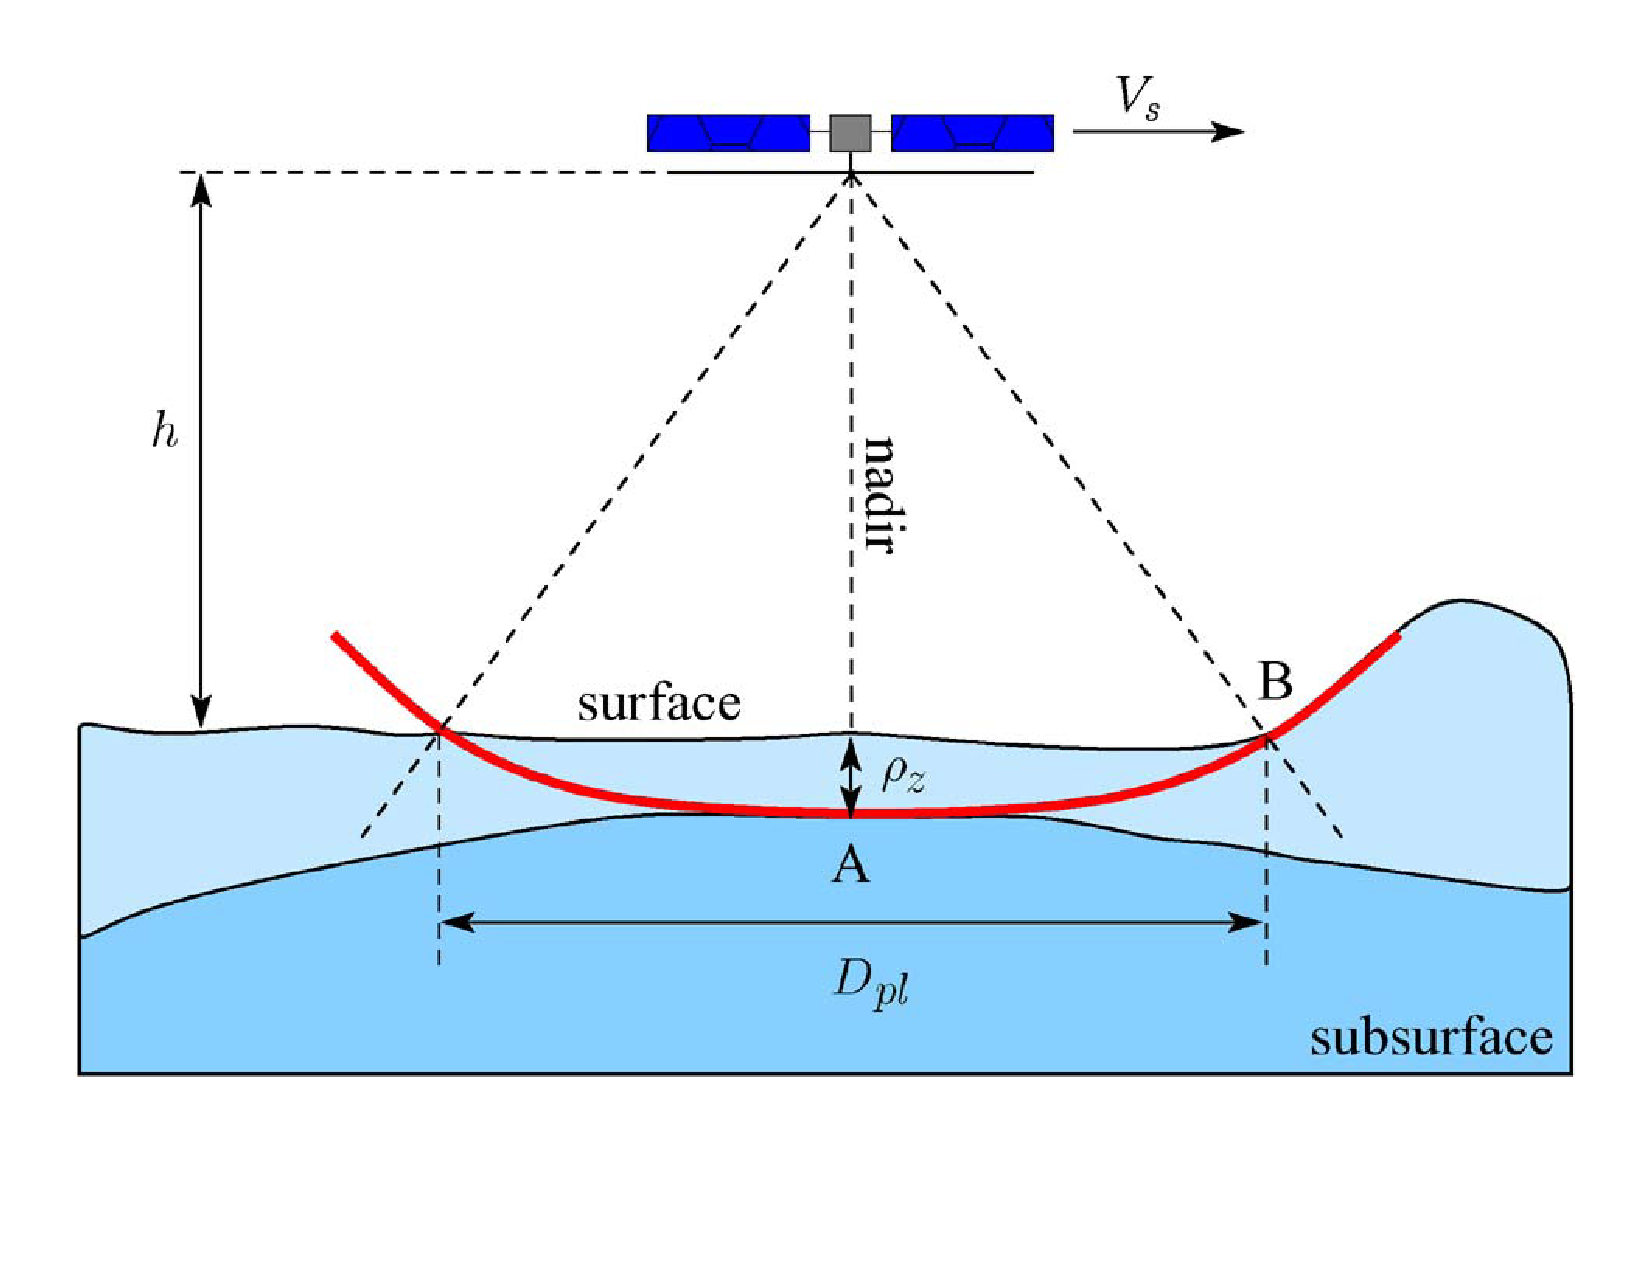
\includegraphics[scale=0.5]{Figures/IPR_Concept.pdf}
\caption{Geometry of \ac{IPR} sounder instrument \cite{Gany_SRS}} 
\label{fig:IPR_concept}
\end{figure}
%
\subsection{Instrument Description}
Architecture of the \ac{IPR} is shown in figure \ref{fig:IPR_achitecture} which is mostly inherited from the SHARAD instrument. It  consists of four main subsystems; \ac{DES}, \ac{TFE}, \ac{RX} and dipole antenna.
\subsubsection{Digital Electronics}
The \ac{DES} is responsible for the radar signal generation. In the design of \ac{IPR}, the concept of software defined radar is utilized with maximum processing in software domain while minimizing the analog electronics. So in order to maintain the high fidelity of the signal, frequency-modulated radar pulses (chirp) are digitally generated directly at the transmit frequency so that no up conversion is needed in the analog domain. A chirp modulated signal will improve the range resolution giving a gain provided by equation \ref{eq:chirp gain} even with low peak power pulses due to hardware constraints.\\
The \ac{DES} is also responsible for all the command and control functions with the spacecraft bus. This controls all the timing sequences of the instrument which are derived from the master oscillator. The instrument will be interfaced to the spacecraft through the \ac{DES} to receive telecommands and for sending telemetries. Also the \ac{DES} provides the processing capabilities for raw data collected during observation and packetizing them into science data packets together with the auxiliary information for ground processing.
\begin{equation}
\eta_{z} = \tau B_{w}
\label{eq:chirp gain}
\end{equation}
%
\subsubsection{Transmitter}
In the \ac{TFE} section, a frequency modulated chirp signal is first amplified to the desired power level and then through the duplexer it goes to the matching network. The duplexer isolates the transmitter from the receiver while permitting the use of the same antenna. A matching network maximizes the radiated power.
%
\subsubsection{Receiver}
The received signal is first amplified by a low noise amplifier and then filtered to reduce the noise in the receiver bandwidth. The amplified signal is converted into the digital domain using an \ac{ADC} and routed to the \ac{DES} where it is down converted and down sampled.
\subsubsection{Antenna}
The antenna for the \ac{IPR} is a 3.6m foldable dipole antenna developed by North Grumrupmam called foldable flattenable tube(FFT). This technology  has been previously used in the \ac{MARSIS} mission. The dipole antenna has a radiation pattern of doughnut shape with the null at the  current feed point.
\begin{figure}[bht]
\centering
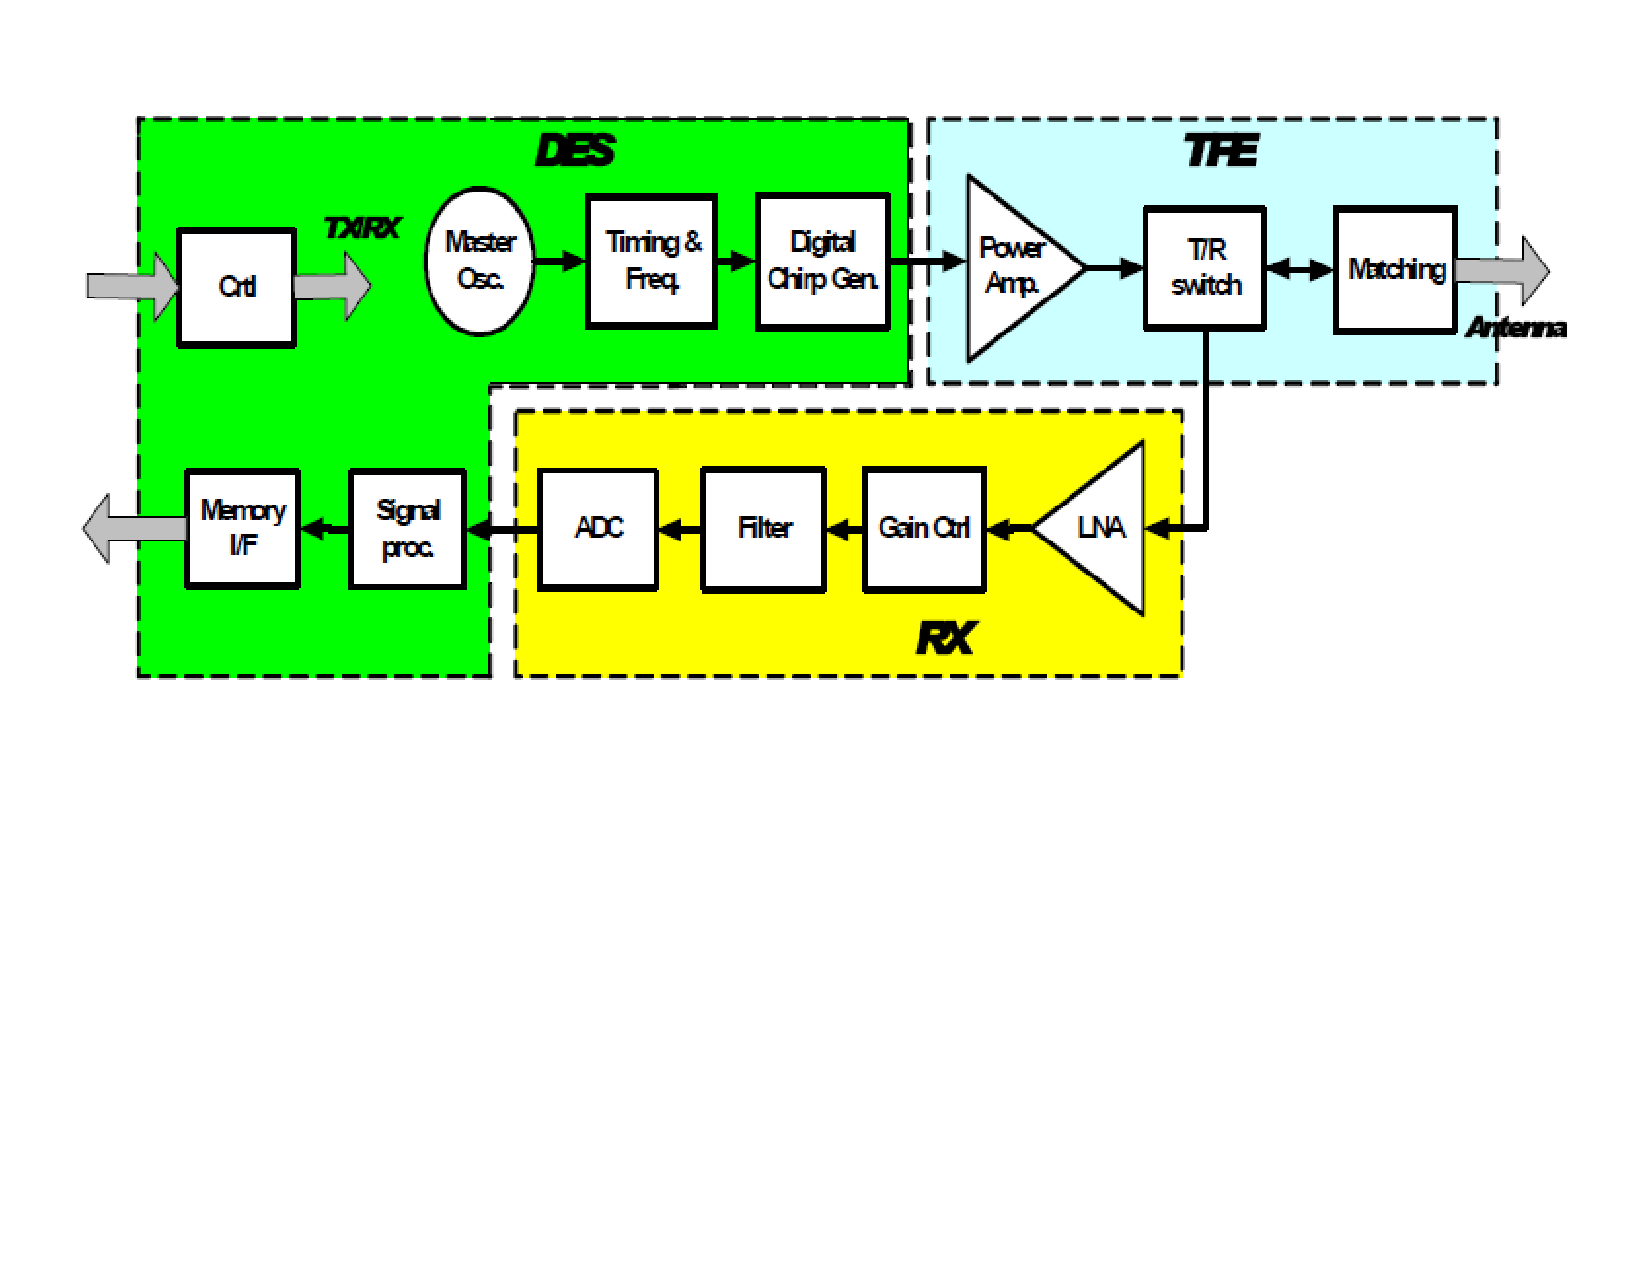
\includegraphics[scale=0.5]{Figures/IPR_Architecture.pdf}
\caption{Architecture of \ac{IPR} instrument \cite{IPR_performance}}
\label{fig:IPR_achitecture}
\end{figure}
%
\subsection{Instrument Characteristics}
The characteristics and parameters of the \ac{IPR} are listed in table \ref{tab:parameter} which are explained in the following subsections.\\

\begin{table}[H]
\centering
\caption{\ac{GIPER} instrument Parameters }
\label{tab:parameter}
\begin{tabular}{|c|c|}
\hline 	\textbf{Parameter}		&  \textbf{Value}\\ 
\hline  Orbit Altitude			&  $200$~km	\\ 
\hline  Centre Frequency		&  $45$~MHz		\\ 
\hline  Chirp Bandwidth			&  $10$~MHz		\\
\hline  PRF						&  $963.39$~Hz	\\  
\hline  Pulse Width				&  $85 \mathrm{~\mu s}$		\\ 
\hline  Ice Range Resolution	&  $8.6$~m		\\
\hline  Along Track Resolution	&  $817$~m		\\ 
\hline  Across Track Resolution	&  $4899$~m		\\ 
\hline  SNR	(surface echo)		&  $26.9$~dB	\\ 
\hline  Power					&  $20$~W		\\ 
\hline  Mass					&  $10$~kg		\\ 
\hline 
\end{tabular} 
\end{table}
\subsubsection{Central Frequency and Bandwidth}
The radar frequency determines the penetration capability of the radar, while the bandwidth of the transmitted pulse determines range resolution \cite{penetrartion}. From the Jovian radiation spectrum as shown in figure \ref{fig:Jovian_radio_emission} measured at 1 AU, it is clear that the frequency cutoff for the Jovian radio emission affecting the subsurface radar is around 40 MHz. So, we choose 45 MHz as central frequency for the \ac{IPR} with 10 MHz bandwidth (40-50 MHz). This gives 3.6~m length for the dipole antenna. Assuming ice ($\epsilon_{r} = 3.2$), Vertical resolution of the \ac{IPR} is 8.4 m which is calculated from equation \ref{eq:range_resolution}.
%
\begin{equation}
\rho_{z} = \dfrac{c}{2B_{w}\sqrt{\epsilon_{r}}}
\label{eq:range_resolution}
\end{equation}
%
\begin{figure}[bht]
\centering
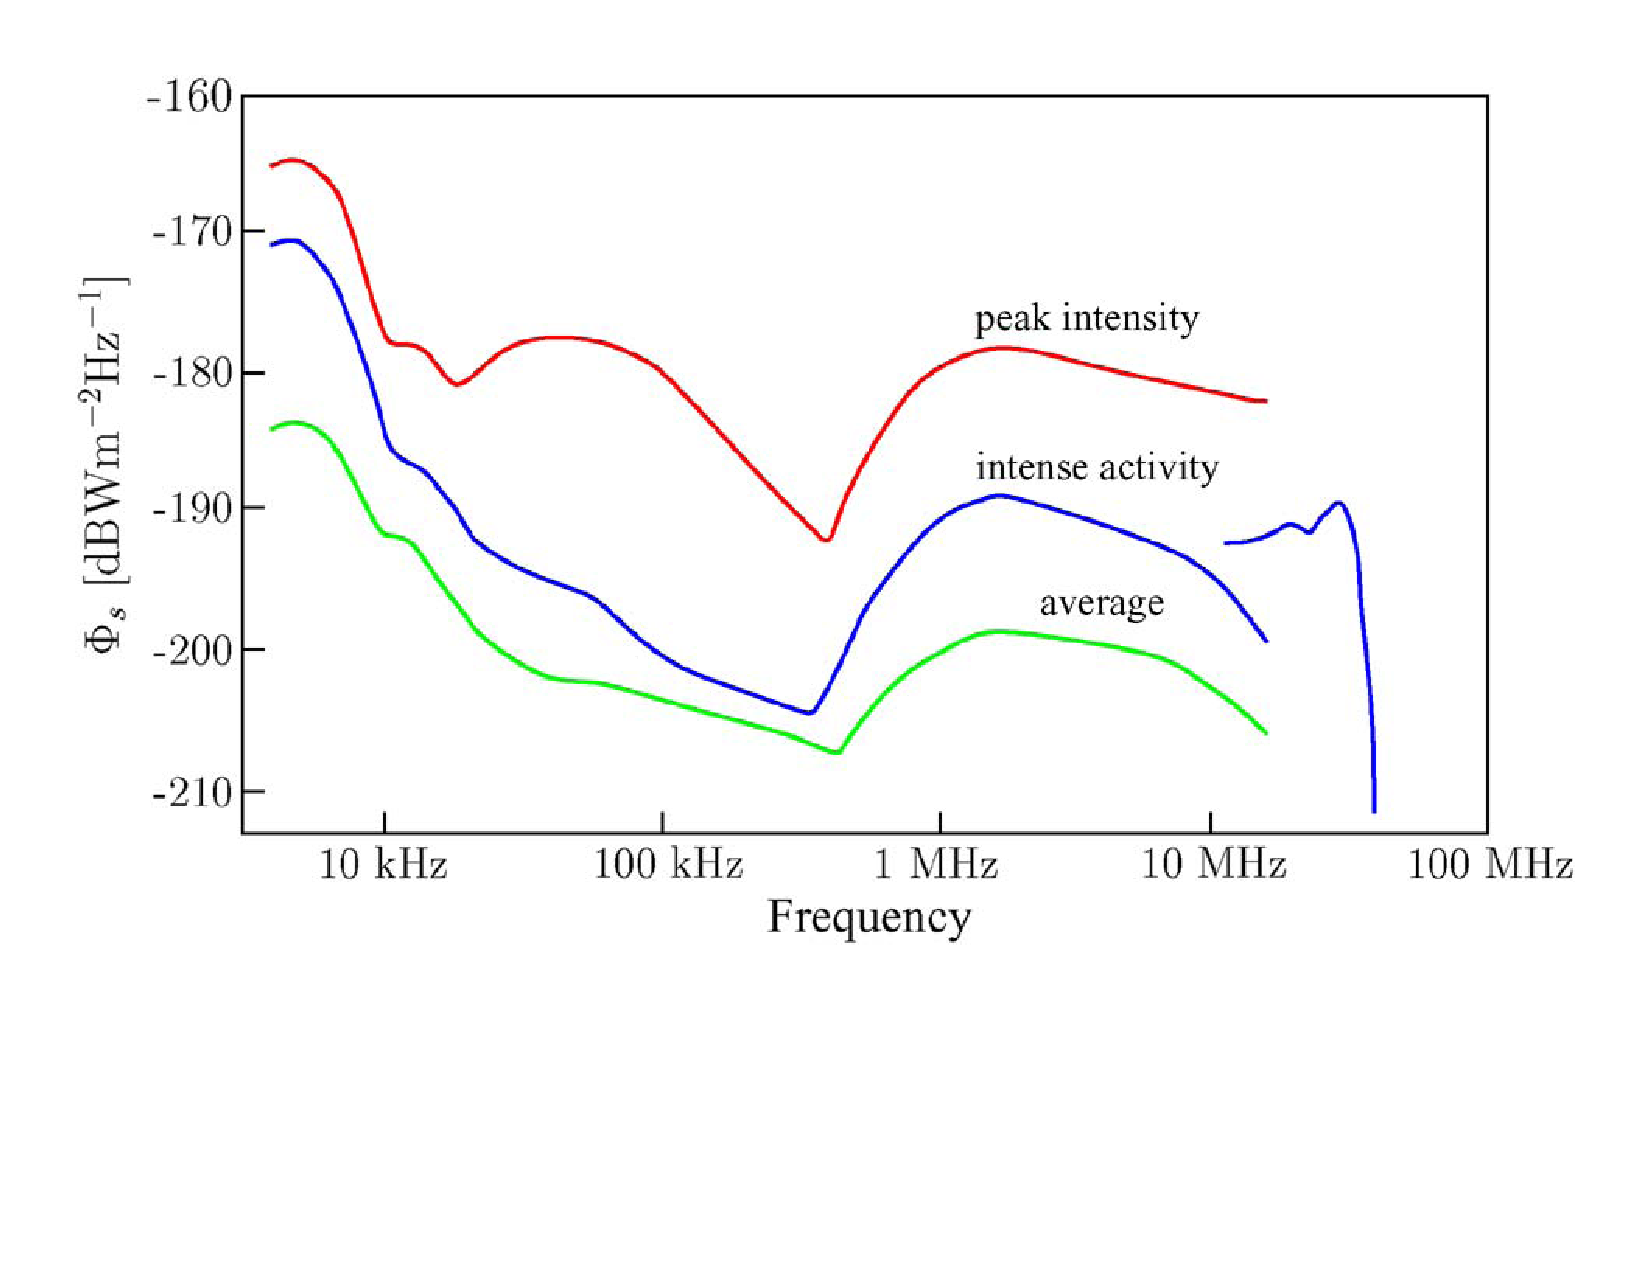
\includegraphics[scale=0.5]{Figures/Jovian_radio_emission.pdf}
\caption{Jovian radio emission spectrum \cite{Gany_SRS}} 
\label{fig:Jovian_radio_emission}
\end{figure}
%
\subsubsection{Pulse Repetition Frequency and Pulse Width}
The pulse width for the \ac{IPR} is $85 \mathrm{~\mu s} $ and \ac{PRI} is $1038 \mathrm{~\mu s}$; giving a duty cycle of $8.2\% $. This results in a \ac{PRF} of $963.39$~Hz. All these timings are shown in figure \ref{fig:PRI}. A receiving window of $165 \mathrm{~\mu s}$ is dedicated to receive the radar echoes. The size of the receiving window is calculated by adding a two way travel time in ice for $5$~km depth ($60 \mathrm{~\mu s}$), the chirp signal duration ($85\mathrm{~\mu s}$) and  a safety margin of $10 \mathrm{~\mu s}$ on each sides. The speed of the electromagnetic waves is reduced by a factor of $1.7$ in ice. A switching time of $177 \mathrm{~\mu s}$ from transmission to reception mode is incorporated as utilized in the \ac{SHARAD} design \cite{SHARAD}.
%
\begin{figure}[bht]
\centering
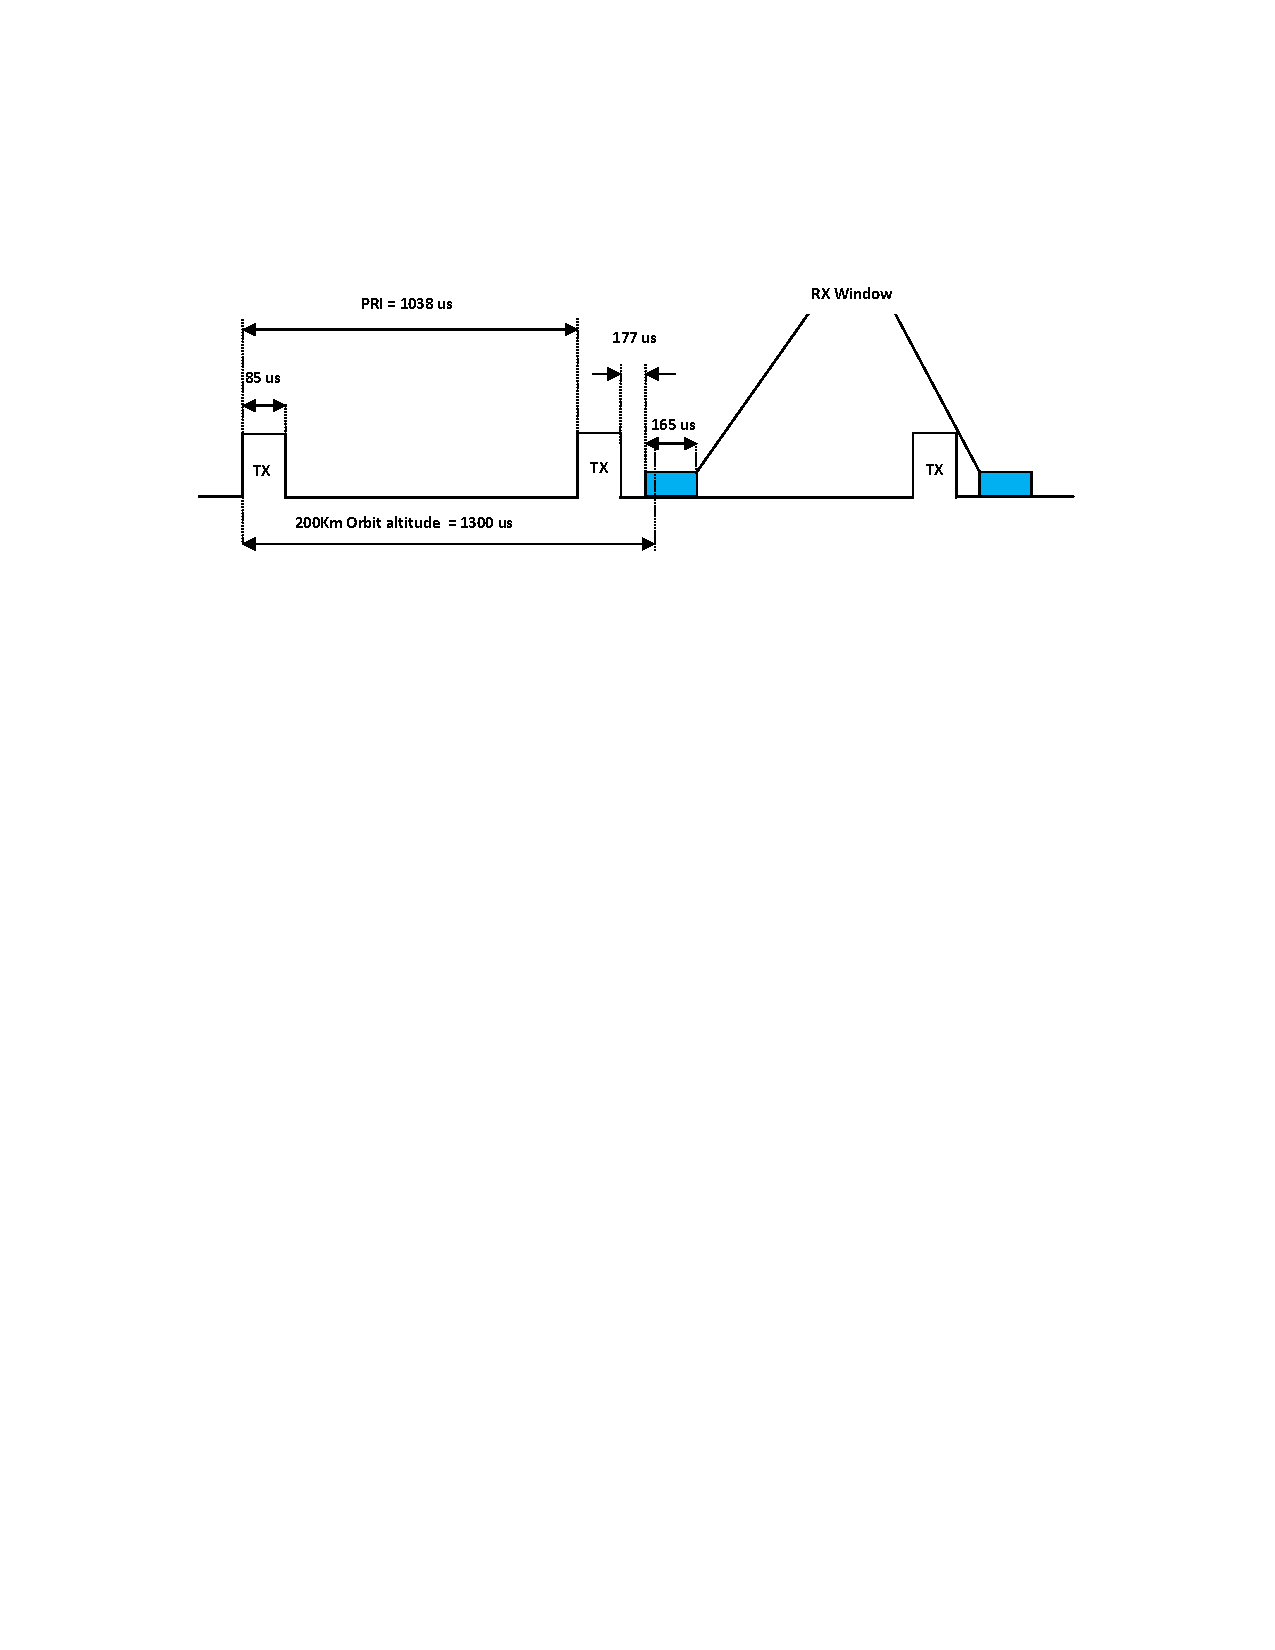
\includegraphics[scale=1]{Figures/PRI.pdf}
\caption{Timing diagram of Ganymede \ac{IPR}} 
\label{fig:PRI}
\end{figure}
%
\subsubsection{Ground Resolution}
%
The resolution of the system is determined by the nature of the target. Over specular surfaces (at the length scale of wavelength), where coherent reflection can be assumed, the resolution becomes that of the ``Fresnel circle'' which is 1633 m calculated using equation \ref{eq:fresenel_circle} from \cite{SHARAD}.
\begin{equation}
D_{f} = \sqrt{2h\lambda}
\label{eq:fresenel_circle}
\end{equation}
where $h$ is the height and $D_{f}$ is the Fresnel circle diameter.

Over rough surfaces, where incoherent scattering is assumed, the ground resolution is approximated with the first pulse limited resolution cell $D_{pl}$ as shown in figure \ref{fig:IPR_concept}. The first pulse-limited cell is represented by a circle on the ground centered in the nadir point, which's diameter is given by the intersection of the wavefront with the ground surface when the transmitted wave has penetrated into the ground to a depth equal to $\rho_{z}$ \cite{Gany_SRS}. So worst case resolution for incoherent scattering calculated from equation \ref{eq:pulse_limited_cell} is 4899 m 
\begin{equation}
D_{pl} = 2\sqrt{\dfrac{hc}{B_{w}}}
\label{eq:pulse_limited_cell}
\end{equation}
However along track resolution can be improved using synthetic aperture processing which is explained in section \ref{SAR} which results in $817$~m using equation \ref{eq:along_track_resolution}. Effective integration time for unfocussed Doppler processing calculated by equation \ref{eq:integration_time} is $860$~ms and the number of pulses used to make synthetic aperture is calculated by equation \ref{eq:Number_pulses} from \cite{Gany_SRS}  which comes out to 666 giving a processing gain of $28$~dB 
%
\begin{equation}
L_{s} = \sqrt{\dfrac{h\lambda}{2}}
\label{eq:along_track_resolution}
\end{equation}
%
\begin{equation}
T_{i,eff} = \dfrac{D_{f}}{V_{s}}
\label{eq:integration_time}
\end{equation}
\begin{equation}
N = T_{i,eff}PRF 
\label{eq:Number_pulses}
\end{equation}
%
\subsubsection{Signal-to-Noise Ratio}
%
The power of the received echo is estimated from the classical radar equation. Using the \ac{IPR} design parameters from table \ref{tab:parameter}, the expected power level of the surface echo is calculated. Here, two processing gains are exploited; one chirp processing gain of $29.3$~dB given by equation \ref{eq:chirp gain} and a second synthetic aperture processing gain of $28$~dB given by equation \ref{eq:Number_pulses}. So after incorporating the processing gain, the signal power from the Ganymede surface is given by equation \ref{eq:radar_basic} which is about $-91.7$~dB
%
\begin{equation}
Pr_{s} = \dfrac{P_{t}\lambda^{2}G^{2}(\frac{D_{pl}}{2})^{2}\sigma_{o}}{(4\pi)^{3}h^{4}} 
	  = -91.7 \mathrm{~dB} 
\label{eq:radar_basic}
\end{equation}
where $P_{t}$ is the transmitted power, $Pr_{s}$ is the surface echo strength $\lambda$ is the wavelength  and $\sigma_{o}$ is the reflection coefficient of the target surface and is a statistical quantity which depends upon the dielectric properties of the two mediums at the interface and can be approximated by the Kirchhoff model \cite{MIMOSA} and for space/ice interface it is equal to $-10$~dB.\\
%
Then the signal attenuation inside ice is estimated. The loss tangent from which the dielectric absorption is calculated depends upon the electromagnetic wave frequency and the temperature of the ice \cite{MIMOSA}. Assuming Ganymede's surface temperature to be 120 K and a slow linear increasing with depth of about 10 K within the first 5~km depth Lorenzo\cite{Gany_SRS} calculated the attenuation of the radar signal for 20 MHz and 50 MHz. Interpolating the result for 45 MHz frequency, the attenuation is $1.2 \mathrm{~dB~per~km}$ giving $12$~dB loss for two way traversing of radar signal in 5~km depth. So any echo after travelling 5~km distance will be $103.7$~dB plus the reflection coefficient of the subsurface layer as given by equation \ref{eq:signal_strength}. The reflection coefficient estimated from the Kirchhoff models for ice/rock and ice/water interfaces are $-11$~dB and -3~dB respectively which is expected for  crater and slush situation as explained in section \ref{sub:volcanism}.
%
\begin{equation}
Pr_{ss} = -103.7 \mathrm{~dB} + 10 \log \sigma_{oss}
\label{eq:signal_strength}
\end{equation}
where $Pr_{ss}$ is the subsurface echo and $\sigma_{oss}$ is the reflection coefficient of the subsurface layer.\\
The radar sensitivity is limited by the noise sources present in the measurement chain. These sources include the Jovian emission, galactic noise and thermal noise of the receiver.  As the central frequency and the associated bandwidth of 10~ MHz is away from the noisy Jovian spectrum so Jovian noise is not critical. Galactic noise temperature at 45~MHz is about $10^{5}$~K while the thermal temperature of the radar receiver will be about  300~K. As, the instrument temperature is quite low as compared to galactic noise, so we can ignore thermal noise of the receiver and the performance of the \ac{IPR} is only limited by the galactic noise which is calculated from equation \ref{eq:galactic_noise} and is equal to -118.6~dB. So signal to noise ($\frac{S}{N_{g}}$) ratio for surface echoe is about 26.9~dB while for the subsurface echo, it will be 11.9~dB and 3.9~dB for slush and crater respectively.
\begin{equation}
N_{g} = K_{B}T_{g}B_{w}
\label{eq:galactic_noise}
\end{equation}
\\
%
%
\subsubsection{Clutter Rejection and Synthetic Aperture Processing}
\label{SAR}
As the directivity of the dipole antenna is quite low, it will illuminate a large surface area of the target. This will result in echoes coming from the off-nadir along with nadir direction as shown in figure \ref{fig:IPR_concept}. This off-nadir echoes called clutter can be divided into two parts; along the track clutter and across the track clutter.\\
%
Along the track clutter will be removed by the synthetic aperture processing technique which uses the relative motion between the spacecraft and target to synthesize a large aperture which is equal to the space covered during the integration time. As the \ac{IPR} is a coherent radar, it measures and records the phase history of the received signals. In order to reduce on board computation and downlink data rate, Doppler processing is chosen unfocused and moreover following the \ac{MARSIS} approach i.e., requiring that the signal phase variation during a synthetic aperture is smaller than $\pi/4$, the phase compensation of the echoes during the formation of a synthetic aperture is simpler and can be performed on board in real time as only a linear phase compensation of the echoes is required \cite{Gany_SRS}. To ensure that only coherently resolved echoes from a contiguous Fresnel zone are being illuminated, the maximum along track integration distance is limited to the Fresnel zone given by equation \ref{eq:
fresenel_circle}.
\\
Across the track clutter is limited by the antenna pattern and will be removed by developing a simulator of the radar using a model of the overflown surface (accurately modelled at the scale of interest), which predicts the presence of clutter echoes. In this way, the corresponding echoes appearing in the measured radar-gram can be properly interpreted as clutter and then be neglected \cite{SHARAD}. Some information for Ganymede was obtained through a \ac{DEM} produced from Voyager images. However, this is not enough  for deriving \acp{DEM} of different portions of Ganymede for a better understanding of the clutter issue \cite{Gany_SRS}. As the instrument package of the \ac{JGO} mission includes radar altimeter so after modelling the Ganeymede surface, across the track clutter will be removed.
%
\subsection{Design Feasibility}
The \ac{IPR} for the \ac{JGO} system is based on a mature and experienced technology that has flight heritage for two different Mars Missions (MARS Express, with the \ac{MARSIS} instrument; NASA Reconnaissance Orbiter with \ac{SHARAD} with slight variations to fullfill  the mission objectives of the \ac{JGO}. From the link budget analysis, it is obvious that we have enough margin to detect the sub layer echoes.  Thus the \ac{IPR} is capable of fullfilling the scientific objectives for the first 5~km surface depth of Ganymede.